\documentclass[10pt]{article}
\usepackage[utf8]{inputenc}
\usepackage{caption}
\usepackage{graphicx}
\usepackage{multicol}
\usepackage[margin=2cm]{geometry}
\usepackage{ragged2e}
\usepackage{amsmath}

\title{\LARGE \bf Tetris Agent Implementation}
\author{Niklas Funk (A0178864J), Madhav Goel (A0179262X), Arijit Pramanik (A0179365N), \\ Simon Schaefer (A0179799U), Svilen Stevanof (A0179092W) - GROUP 33} 
\date{\vspace{-5ex}}

\newenvironment{Figure}
{\par\medskip\noindent\minipage{\linewidth}}
{\endminipage\par\medskip}

\begin{document}

\begin{center}
Introduction to Artificial Intelligence - CS3243 - National University of Singapore \\
21 - 04 - 2018 
\end{center}
\vspace*{-4em}

{\let\newpage\relax\maketitle}
\maketitle
\thispagestyle{empty}
\pagestyle{empty}

\parindent 0pt

\begin{multicols}{2}
\begin{abstract}
\bfseries
This report is about the challenge of designing an utility based agent which can maximize the number of rows cleared in the game of Tetris. We achieved the best performance using a genetic algorithm but also present other approaches. 
\mdseries
\end{abstract}
\section{Introduction}
\label{sec:problem}
The game of Tetris has seven distinct block shapes (Tetraminos), which can be manoeuvred by translation or rotation. The ultimate goal is to place the Tetraminos such that the number of cleared rows is maximized and that, in theory, the game never terminates.  
\newline
The Tetris game is fully observable since the complete board is known at any point in time. It is sequential and static, as the orientation of Tetraminos merely changes as a consequence of the player's moves. The game is discrete as it acts in a discrete 20x10 grid. Though each action is deterministic, while the choice of the next Tetramino is randomly distributed over all seven shapes.
\newline
The next player move can be determined using a utility based agent. Its utility function is a weighted sum of different features of the board for a given state, which can be determined using genetic algorithm. The following section gives a detailed overview of our implementation.
\vspace{-0.8cm}
% Tetris is a popular computer game invented by Alexey Pajitnov in 1985, played on a 20x10 rectangular grid and filled by Tetraminos (seven distinct shapes of blocks). The player maneuvers the blocks by rotation and translation to place them on the board. When a row of is fully occupied it is removed. The objective of the game is to clear as many rows as possible.
% \newline 

\section{Genetic Algorithm}
\label{sec:genetic}
\vspace{-0.45cm}
Genetic algorithms are search algorithms based on the mechanics of natural selection and genetics as observed in the biological world. They use both, “survival of the fittest” and "mutation" (randomization) to robustly explore the best choice of weights.

%\subsection{Pipeline}
%Diagram of the genetic algorithm architecture and description how the code runs 
\vspace{-0.4cm}
\subsection{Features}
To determine the next move, all possible move are compared using a utility function and the move resulting in the highest utility is chosen. The utility function is a weighted sum of different, state-dependent, human engineered features. A "good" choice of features therefore is crucial in order to obtain a well-performing agent.
\newline 
The current state is defined by the occupancy of the board and the next Tetramino. One can also define abstract state descriptors like the height of columns, holes, wells and transitions. A hole is an empty cell with an occupied cell above it. A well is a column whose adjacent columns are higher than it, and its depth is defined as the difference of the height of well column and the shorter adjacent column. Transitions are the number of empty-occupied cell switches in the respective column or row. The final set of features we used are: 

\begin{enumerate}
\itemsep0em 
\item Sum of height differences between adjacent columns.
\item Maximum height of a column.
\item Total number of cleared rows.
\item Whether the current move results in a loss.
\item Total number of holes. 
\item Sum of depths of all wells in the game board.
\item Mean of the absolute difference between the height of each column and the mean height
\end{enumerate}
\vspace{-0.45cm}
%Initial state, crossing over and mutations
\subsection{Training Algorithm Implementation}
In order to find an optimal set of weights, several steps are repeated iteratively: First, an initial population of randomly drawn weight vectors from a uniform(0, 1) distribution is generated. 
\newline
To produce the subsequent generations, we first choose a parent in the following way: We calculate the sum of scores of all members of the previous generation and multiply it with a random number from a uniform(0,1) distribution to define a threshold value. We then randomly draw members from the previous generation and check if their score crosses the threshold value. If it does, we choose that member as as a parent. Else we reduce this threshold and continue the search by drawing a different member from the population. In case no member of the previous generation crosses the threshold, we return the member with the highest score in the previous generation as the parent.
\newline
After selection two parents using the above method, we use the single point crossing over heuristic to determine the weights of the two children produced. In this heuristic, a single crossover point on both parents' weight sequence is selected. All weights beyond that point in the parents' weight sequence is swapped between the two parent organisms to generate the two children. We used a 0.6\% crossing-over rate. The rate defines the probability for the crossing over to happen. In case crossing over does not happen, the parents chosen are directly passed as children to the next generation.

Subsequently, each weight of the child can undergo mutation with 1\% probability. If a mutation occurs, the specific weight is multiplied with a uniformly drawn value between 0.8 and 1.2.

\subsection{Parallel Processing}
Due to the randomness in the choice of next stone, each game is different. In order to avoid "overfitting", i.e. a set of weights merely performs well for a specific sequence of stones, the score for each member is the average score of 10 games. As these games are independent from each other, they are played in parallel, using multi-threading. Similarly, each member of the population has its own set of independent feature weights and hence, they are also evaluated leveraging multi-threading.
This achieves a speedup of roughly 10.82, e.g. given a population size of 50, the multi-threaded version needs \texttt{7m53s} per generation while the older version needed \texttt{85m19s}.

\subsection{Results}
We analyze the results from 100 runs of the game using the weight vector $\vec{w}$ shown right below, which were derived training our best genetic algorithm for 200 generations with a population size of 40. The weights of the features are ordered as in Section 2.1. 

$$\vec{w} = 
\begin{bmatrix}
0.69, -0.60, 0.80, 1.07, 0.68, 1.13, 3.63
\end{bmatrix}$$

Figure \ref{fig:graph_100_runs} gives us the distribution of the performance results from 100 iterations. We observe that while most results are below 100,000 rows cleared, there are 10 iterations where we clear more than 200,000 rows.  

\centering
\begin{tabular}{| l | c |}
\hline
\textbf{Metric} & \textbf{Value} \\
\       hline
Average & 119,560 	\\ \hline
Median & 82,706 		\\ \hline
Maximum & 864,157 		\\ \hline
Minimum & 101		 	\\ \hline
\end{tabular}
\captionof{table}{Performance of best weights over 100 iterations}
\justify

Table 2 shows us that the while the minimum number of rows cleared is 101, we clear a maximum of 864,157 rows. The average number of rows cleared is 119,560 which is cleary higher than the median of 82,706. This aberration is due to our extremely well performing runs when the sequence of incoming stones is very beneficial to our set of weights.

Figure \ref{fig:mean_median_graph} shows that there is a linear relationship between the mean and the median of the 10 best results of each generation during training. This means that we don't get random outliers of weights which give good scores for very few members while all others perform poorly. Instead we have a smooth development and increase of the performance during training. Also, the graph shows that the mean scores during training are lower for population sizes of 15 and 25, and increases significantly for population sizes greater than 40. The performance tends to converge for population size 40, as there isn't any improvement with population size 100. This means that the population size has to pass a certain threshold such that the random processes of crossing over and mutation are likely to "produce" significant improvements.

\begin{Figure}
\centering
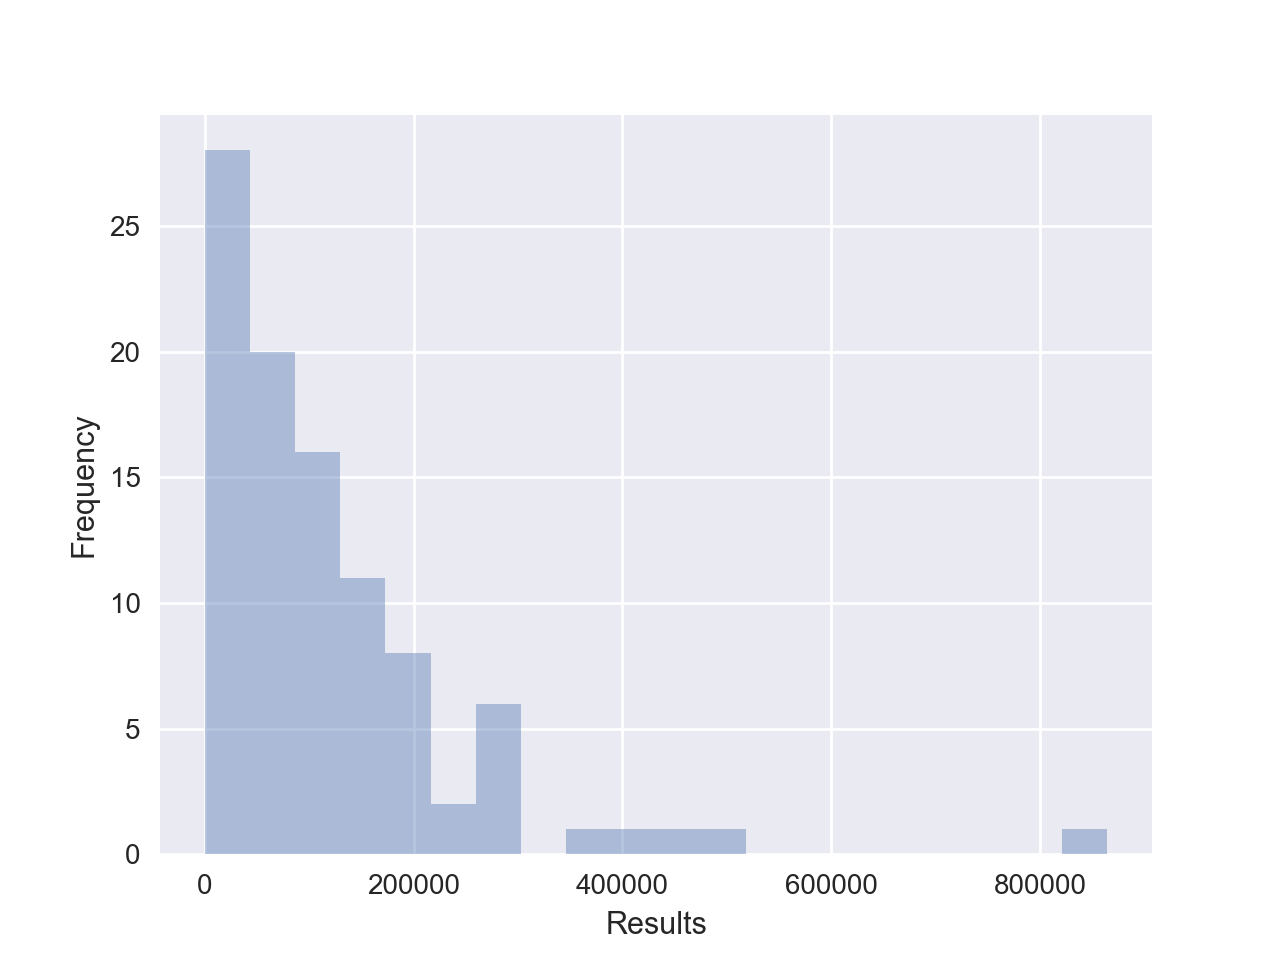
\includegraphics[width=8cm]{imgs/Results_Hists.png}
\captionof{figure}{Results from 100 iterations of the game}
\label{fig:graph_100_runs}
\end{Figure}

\begin{Figure}
\centering
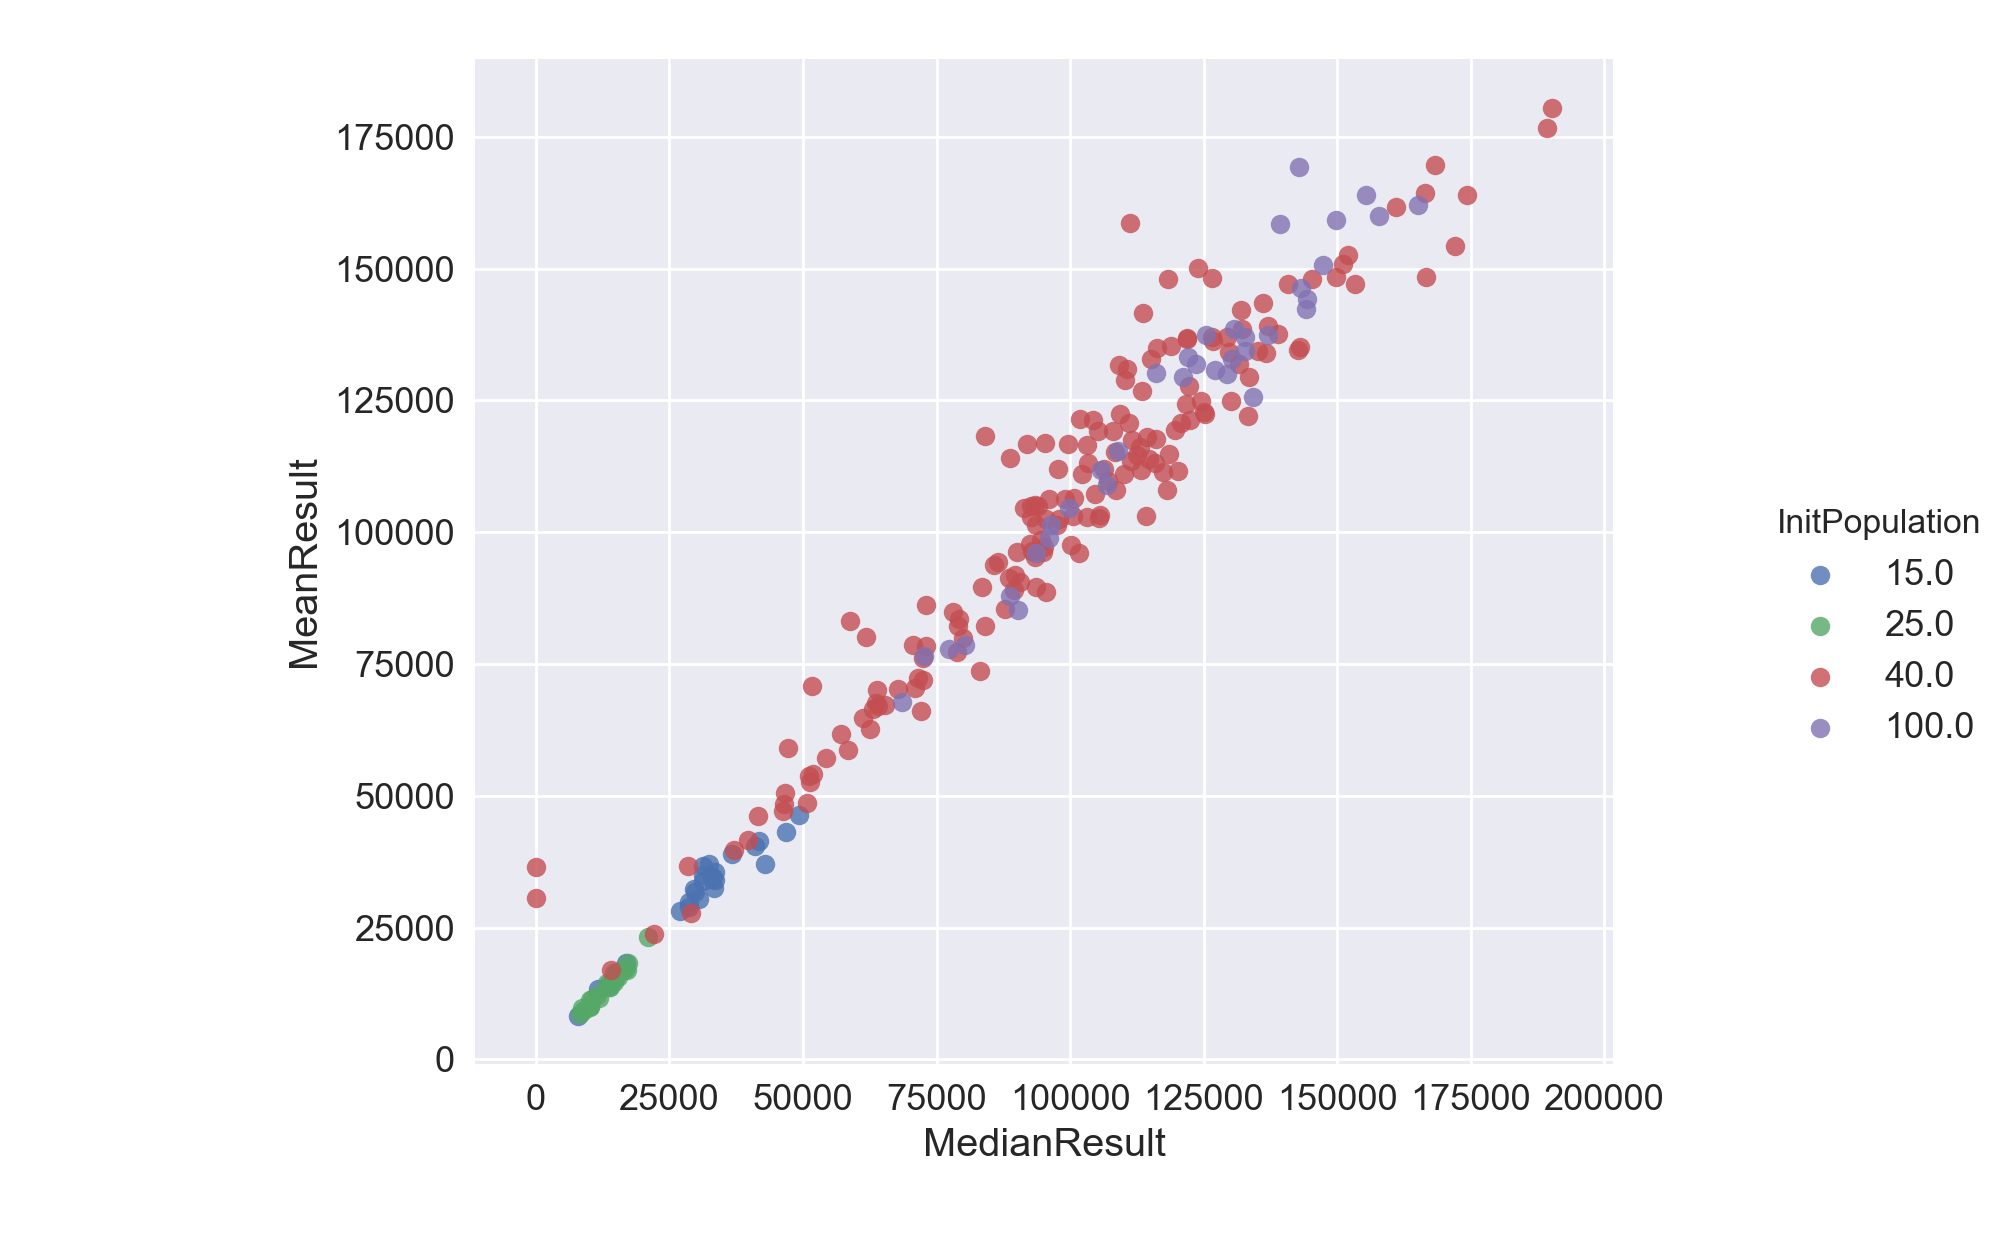
\includegraphics[width=8cm]{imgs/Median_Mean.png}
\captionof{figure}{Mean-Median plot of intermediate scores during training for different population sizes.}
\label{fig:mean_median_graph}
\end{Figure}

% \subsection{Analysis}
% W
% ...\textit{Which performs best ?}

% Maybe we can say that we don't have amazing results because we didn't train it enough since we thought that there was a problem in our approach. We thought that because of the results of others (cite other papers) 
\section{Further Experiments}
\subsection{Additional Features}
We tested out several other features, but discarded them later as they did not improve results. They were: 
\begin{enumerate}
\itemsep0em 
\item Number of connected holes.
\item Difference between maximum and minimum column height.
\item Maximum depth of well. 
\item Number of blocks currently present on the board.
\item Weighted number of blocks, where you penalize blocks in proportion to the height at which it is located.
\item Number of Horizontal transitions.
\item Number of Vertical transitions.
\end{enumerate}

\subsection{Other heuristics for crossing over}
We experimented with some other heuristics for performing the crossing over of the two parents to generate the child :
\begin{enumerate}
\itemsep0em 
\item The child randomly picks the full set of weights of one of its parents 
\item The child's weights are average of weights of the parents
\item For each feature, the child randomly inherits the weight from one of the parents
\item Generate a random number k, and the child takes the first k weights from one parent and the rest from the other
\end{enumerate}
However, we got a maximum of 86,516 cleared rows with these other heuristics and thus discarded them. Graphs for analyzing performance of these heuristics can be found in the appendix.


% \subsubsection{Alternative Training Algorithm}
%  We experimented with the method for performing the crossing over.
% \newline
% To formulate a new generation, 30\% of the best performing parents from the previous generation are directly passed as children, while the remaining 70\% of the population is generated as follows :
% \newline
% Randomly a subset (25\%) of members from the previous generation is chosen. Then from this subset the member with best performing set of weights is chosen as the first parent. The other parent is picked from a different subset, using the same approach. 
% \newline
% After the parents have been selected, a heuristic defines how to perform the crossing over, i.e. how the child evolves from its parents. During the project, there were several heuristics that we tested: 


% We also designed a fitness function which checks if the newly generated child performs as least as good as the worst child so far in the population. If this isn't the case, it is replaced by a newly generated child that results from another crossing-over process. To avoid infinite loops, an upper limit for the number of children which can be rejected is fixed to 5. 

\subsection{Particle Swarm Optimization (PSO)}
PSO is a computational method that iteratively tries to improve a candidate solution with respect to a given measure of quality. At each iteration, it keeps track of the best feature weights for every population member, and also for the entire population. We modify the weights at each iteration, influenced by the best weights for that member as well as for the entire population, using the velocity vector for each feature, and update them in case a personal best or global best set of weights is found(which clears the most number of rows). This optimization directs the movement of weights of the future generations based on memory of best performing members of the previous generations. This helps converge the current genetic agent candidate towards the most optimal one found so far.

\subsection{Other Algorithms}
Using a genetic algorithm is capable of finding a well-performing solution but still heavily depends on the features engineered by humans. Thus, we tested data-driven algorithms in order to eliminate the necessity of human feature engineering.  

\subsubsection{Q Learning}
Q Learning is a kind of reinforcement learning, that does not require a model of its environment. For each game state ($s$), Q Learning maps all possible actions ($a$) to rewards $Q(s,a) $. The Q function's values for each pair $(s,a)$ is derived during training procedure, using the Bellman equation \cite{qlearning}: 

$$Q(s,a) = r + \gamma \max_{a'} Q(s', a')$$

Meaningly, the reward for taking action $a$ in state $s$ is the sum of the initial reward of this action $(r)$ and the weighted reward of the next state $s'$. In order to get a Q value for all actions in every state, during training time, a random action is chosen with probability $\epsilon = 0.4$. Otherwise, the greedy policy determines the action. The training is terminated when all of the Q-values converged. This might include to have a decreasing learning and random move picking rate ($\gamma$ resp. $\epsilon$). 
\newline
The Q-learning approach is therefore in need of a reward function (r) but in contrast to the genetic algorithm approach this is very intuitive e.g. for Tetris, $r=-1$ if the game has ended and $r=0$ otherwise is sufficient, or for CTB, $r=1$ if the ball was cought and $r=-1$ if the ball passed the catcher (see chapter \ref{sec:generality}). 

\vspace{0.25cm}

Therefore the Q learning method is capable of playing any game without any a priori knowledge about the environment, only terminal state games have to be assigned a "reward". Nevertheless a lot of training iterations are necessary until all of the Q values converged and have been updated at least once. While this does not pose a problem in case of small states and action spaces, as in the CTB game with $\mathcal{O}(10^2)$ possible pairs, indeed the Q learning training procedure is infeasible in case of large state spaces. The Tetris as characterized in \ref{sec:problem} has $2^{200} = \mathcal{O}(10^{60})$ states. Even if one training iteration would take less than a nanosecond and the algorithm would never revisit states updating every entry in the Q matrix would require roughly $10^{43}$ years. It can nevertheless be shown that the Q learning approach works in the Tetris frame. For a simpler version of Tetris \footnote{The simpler Tetris game differs from the "standard" Tetris game in matters of both the board size (3x3) and the set of Tetraminos (2) used, in order to reduce the space-action-space.} the Q values converged after 10000 iterations and afterwards the agent clears an infinite number of rows. Thus, to solve the "standard" Tetris game with a Q-Learning approach, the challenge is to narrow the state space dramatically and reasonably. 

\vspace{0.25cm}

For the purpose of shrinking the state-space several approaches were tested. Most of our approaches resulted in a too large loss of information and consequently to a very bad performance of the agent (e.g. redefining the game's state as the top (two) rows of the board). 

\subsubsection{Auto Encoder}
High-dimensional data can be converted to a lower-dimensional representation by training a multilayer neural network. This network (see figure \ref{fig:encoder_arch}) is symmetric with respect to the small central layer (whose output is the encoded input). Therefore the first part of the network encodes the data, while the second one decodes it and the resulting error is used to optimize the networks' weights (\cite{autoencoder}). In the Tetris game an auto encoder can be used to encode the field (state) and replace it by a low-dimensional column vector. 

\begin{Figure}
\centering
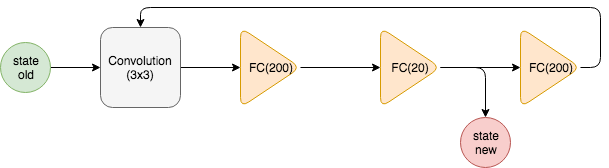
\includegraphics[width=8cm]{imgs/encoder_structure.png}
\captionof{figure}{Auto Encoder - Architecture}
\label{fig:encoder_arch}
\end{Figure}

To represent the Tetris board in a lower-dimensional space the adjacent structure of every cell (e.g. holes) could be important. Hence, the board is convoluted first and the convoluted board is fed into the autoencoder which consists of three fully connected layers, down-sampling to a vector of size 20, and is trained using batch-normalized stochastic gradient and subsequently steepest gradient descent, to avoid getting stuck in a local minimum (compare \ref{fig:encoder_errors}). For building and training the network the encog framework \cite{encog} was deployed.

\subsubsection*{Auto Encoder in Genetic Algorithm}
Instead of manual feature engineering the features could be derived by learning a shrunk state representation, i.e. by using the auto encoder's state directly. We used our CTB implementation to first verify this new general idea. To perfectly perform in the CTB game (section \ref{sec:appendix}) merely the distance between catcher and ball is necessary as a state, a full state description is given by the distance and a position of either the catcher or the ball (merely x-coordinate regarded here). In theory the game's internal state, i.e. two hot-encoded vectors containing the discrete x-position of both catcher and ball, should be down-sampled to this smallest possible state description. Unfortunately, applying an autoencoder to the CTB game results in two values that are not separately dependent on either the distance or position but contain a combination of both. Thus, even if the encoder's output well defines the game's state, it can nevertheless not be used as feature vector, since the agent's decision should surely not be affected by the absolute position of catcher/ball in the CTB example. In general the previously described problem arises as well when applied on the Tetris game. Hence, the genetic agent trained with autoencoded features did not perform well for the two games.

\section{General Agent}
\label{sec:generality}
Another goal of our project was to design the agents in a general style such that they are not limited to only playing Tetris, but can be easily deployed and tested on CTB or any other game which is implemented in line with our abstract (general) game class. The roadbloack here is that we have not yet found an algorithm which can automatically calculate reasonable set of features. Therefore human "feature engineering" will still be required. 

\begin{Figure}
\centering
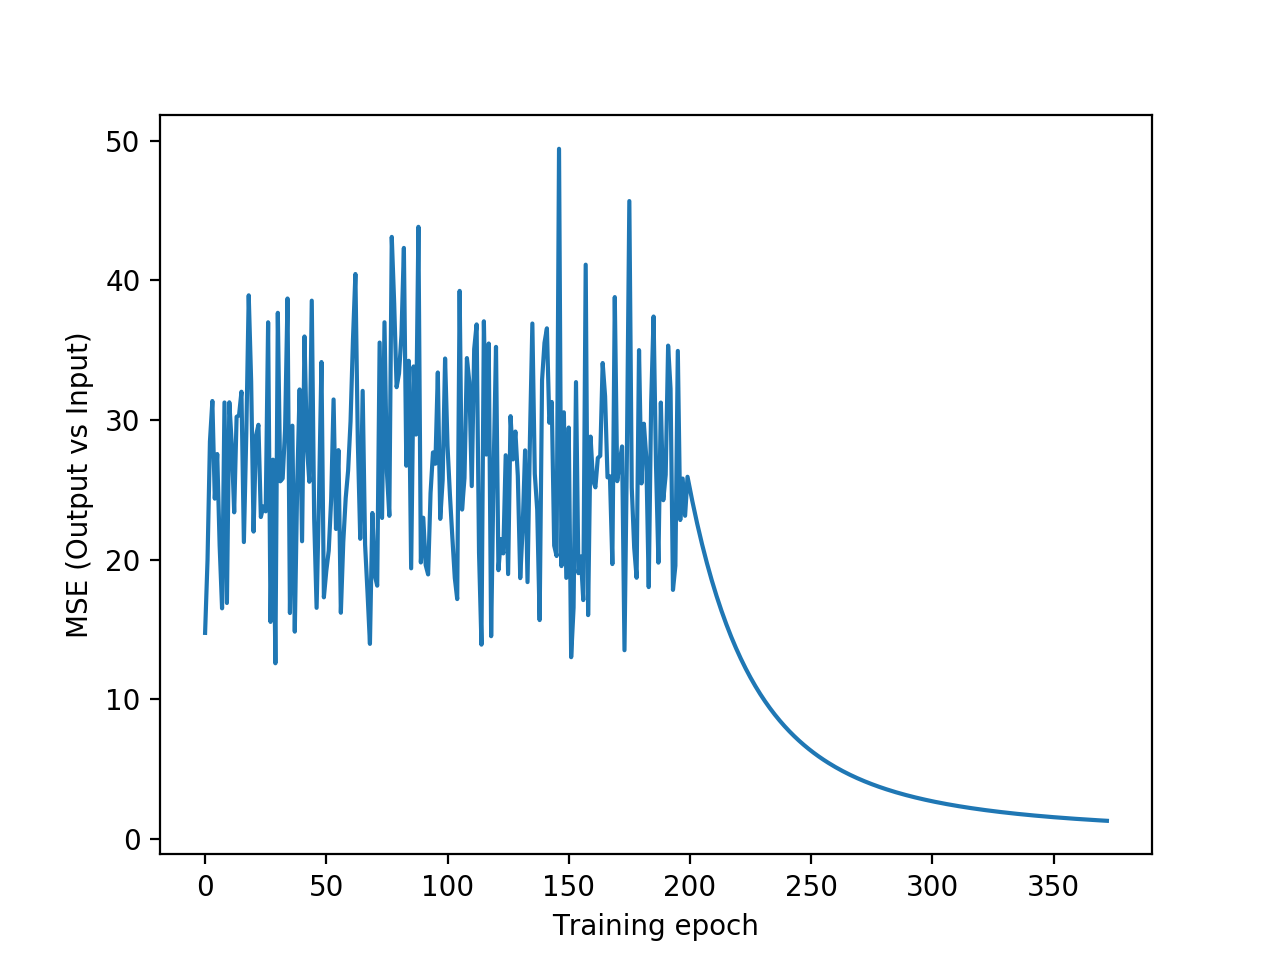
\includegraphics[width=6cm]{imgs/encoder_errors.png}
\captionof{figure}{Auto Encoder - Training errors}
\label{fig:encoder_errors}
\end{Figure}

% \subsubsection*{Auto Encoder - Q Learning}
% Although the auto encoder described above manages to down-sample the state-space dramatically its output is not discrete, as required for the Q learning approach. In order to apply a Q learning based approach deep Q learning would have to be used, which is behind the scope of this project.

  

\section{Discussion}
\label{sec:discussion}

Future improvements include making the genetic agent more robust by looking one move ahead and factoring that in to decide the best current move. Also, one could try to find a state space representation suitable for playing Tetris with the Q-Learning approach. Overall, we are pretty satisfied with our results, especially considering the amount of time and effort we invested in exploring the Q-Learning and the Autoencoder approach.  We were able to scale our algorithm to use big data, since the genetic algorithm has an inherent structure for parallelization. Our implementation using multithreading was able to execute 86 generations of the genetic agent with a population size of 100 in about 5 hours using the 10 cores on the NSCC cluster achieving a mean cleared rows of about 118,587. 
\newline
\newline
The genetic algorithm and PSO optimization parameters required extensive tuning, and given the limited time, we focused on tuning the heuristics for crossing over and mutation rate, along with different population sizes, since this helps in achieving a better population in fewer generations. We also tried tuning the weights of velocity and coefficients of influence of the local and global best results for the population using PSO. But this only led to marginal improvement in results. The genetic algorithm evolves quite steadily, but slowly in the solution space, while the PSO occasionally gives good results. Hence, we thought of combining the two so that any good set of weights in the solution space obtained randomly could be converged upon. This is evident of the fact that genetic algorithm tends to localize to a suboptimal solution and exploit the solution space, while PSO tends to explore it. A higher velocity coefficient explores the search space more. So, the search problem is essentially balancing between exploitation and exploration, which could have been improved by applying PSO on a fraction of the population. We observe a large variability in the results, as is inherent in mutation, selection threshold of parents and initial set of random weights of the population and velocities imparted to the features. 



\end{multicols}

\newpage
\begin{multicols}{2}
\section*{Appendix}
\label{sec:appendix}

\subsubsection*{Catch the Ball (CTB)}
The Catch the Ball (CTB) game consists of two objects, a ball and a catcher. In each turn the ball's and catcher's horizontal position are randomly initialized. Then, the ball is straight falling down from its starting position and the player has to adapt the catcher's horizontal position (via 3 inputs: move left/right or stay) so that the ball is "captured" (i.e. $x_{ball} = x_{catcher}$). The visual representation of the CTB game is shown in \ref{fig:catch_the_ball}. 

\begin{Figure}
\begin{center}
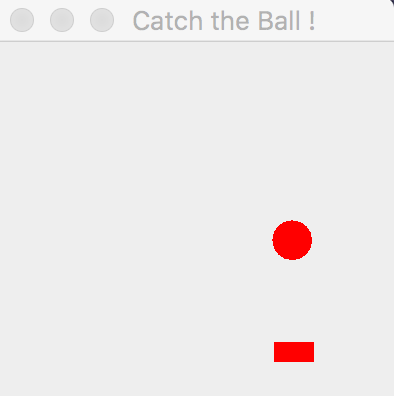
\includegraphics[width=4cm]{imgs/catch_the_ball.png}
\end{center}
\captionof{figure}{Test game - Catch the Ball.}
\label{fig:catch_the_ball}
\end{Figure}

In CTB the possible states are defined by the discrete distance between catcher and ball, which results in $2 width_{board}$ states. Combined with three actions (moving left, right or staying) we have 600 possible state-action-pairs, assuming a game board with of 200. Here, after roughly 10000 training games a well defined Q(s,a) matrix is obtained resulting in a well-performing agent.

\subsection*{Further Diagrams}


\begin{Figure}
\begin{center}
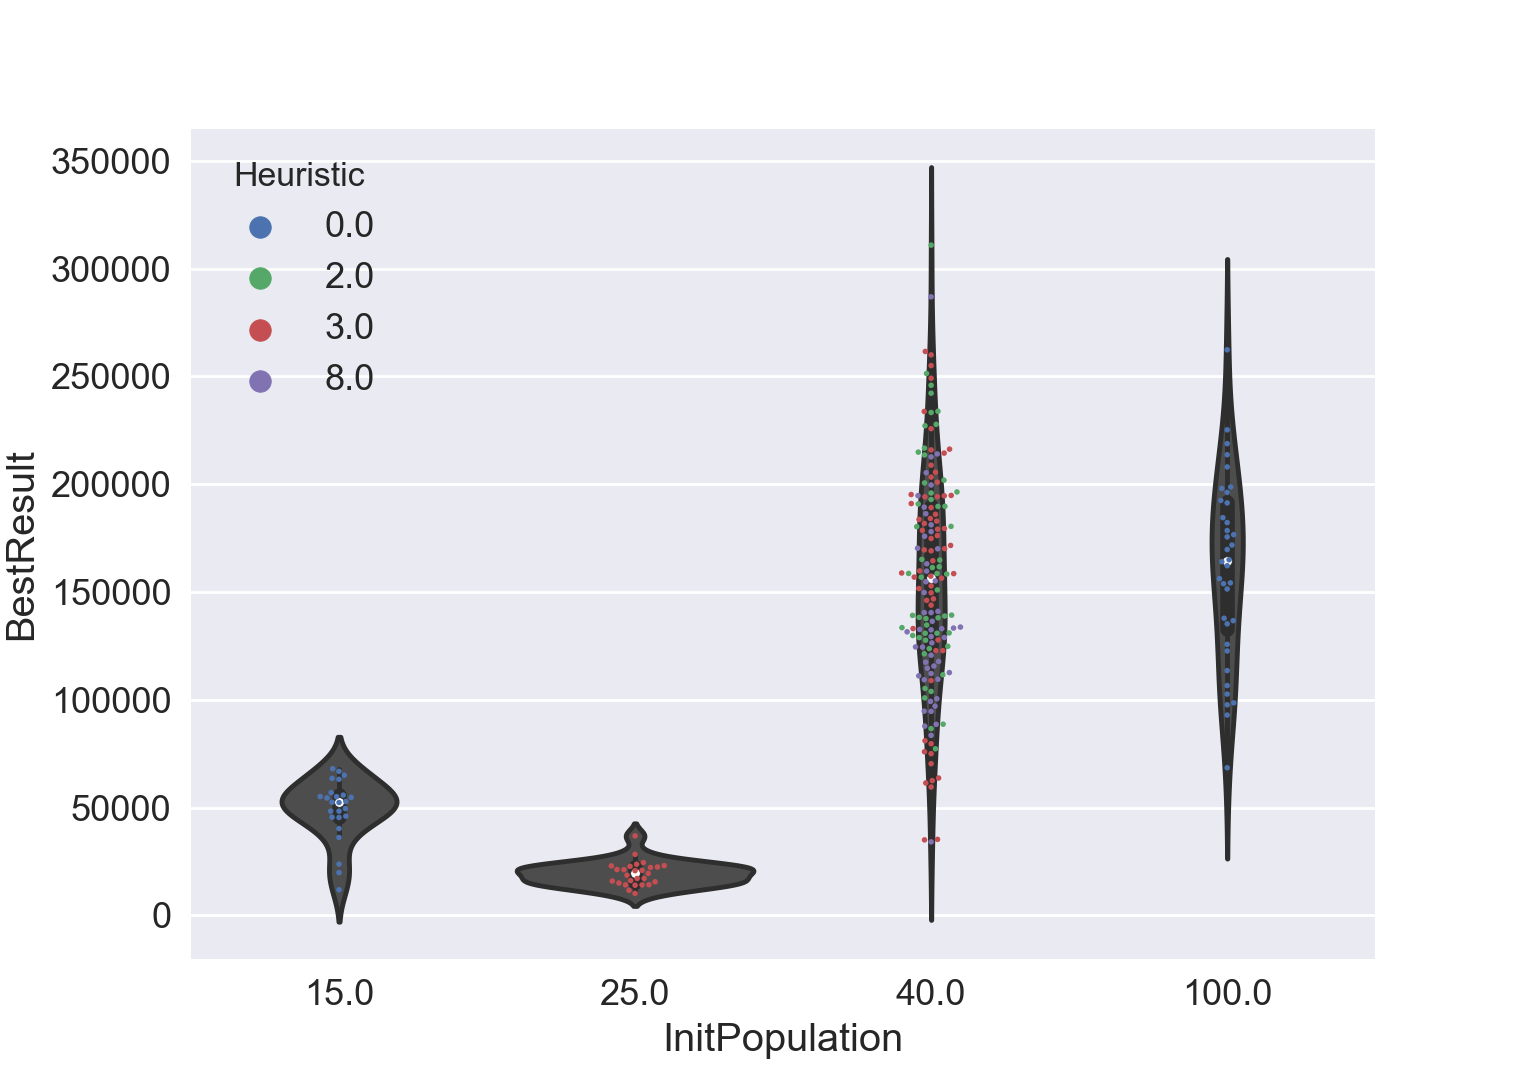
\includegraphics[width=7cm]{imgs/InitPop_Best.png}
\end{center}
\captionof{figure}{Comparison of initial population.}
\label{fig:initpop_best}
\end{Figure}
\begin{thebibliography}{9}
\bibitem{autoencoder} 
G. E. Hinton* and R. R. Salakhutdinov.
\textit{Reducing the Dimensionality of Data with Neural Networks}. 
Science, 2006.

\bibitem{encog} 
J. Heaton.
\textit{Encog Machine Learning Framework}. 
Heaton Research, 2018.

\bibitem{qlearning}
C. Watkins. 
\textit{Technical Note: Q-Learning}. 
Kluwer Academic Publishers, 1992.

\end{thebibliography}
\end{multicols}

\end{document}